\documentclass{standalone}

\usetikzlibrary{arrows,positioning, shapes.geometric}

\def\layersep{0.65cm}
\def\xconnection (#1,#2) {\draw[connection] (#1.north west) -- (#2.south east);  \draw[connection] (#1.north east) -- (#2.south west);}
\def\connection (#1,#2) {\draw[connection] (#1.north west) -- (#2.south west);  \draw[connection] (#1.north east) -- (#2.south east);}
\def\oconnection (#1,#2) {\draw[connection, dashed] (#1.north west) -- (#2.south east);  \draw[connection, dashed] (#1.north east) -- (#2.south west);}

\begin{document}

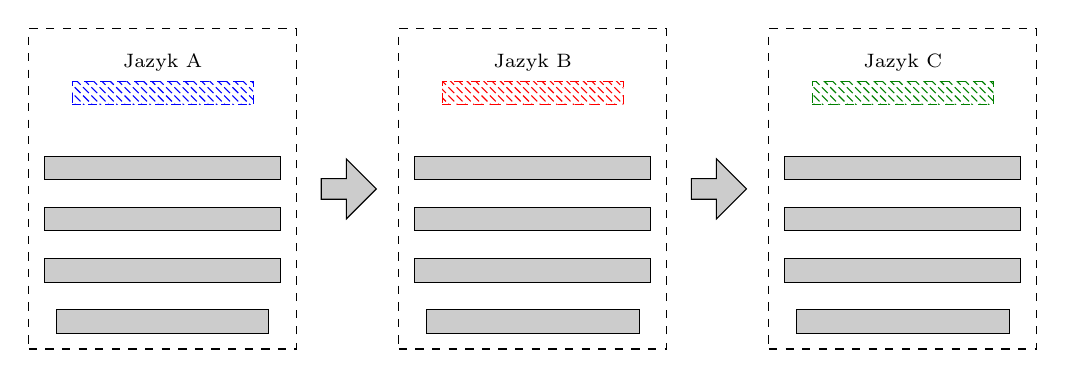
\begin{tikzpicture}[draw=black, node distance=\layersep, every node/.style = {font=\scriptsize}]
	\usetikzlibrary{patterns, fit, arrows.meta, positioning, shapes.geometric, calc, shapes.arrows, shadows, backgrounds}
    \tikzstyle{layer}=[rectangle, draw=black, fill=gray!40, minimum height=0.3cm, line width=0cm]
	\tikzstyle{hidden layer}=[layer, minimum width=3cm]
	\tikzstyle{input layer}=[layer, minimum width=2.7cm]
	\tikzstyle{output layer}=[layer, dashed, pattern=north west lines, pattern color=gray, minimum width=2.3cm]
    \tikzstyle{annot}= [text width=4em, text centered]
	\tikzstyle{connection}=[ thin]
	\tikzstyle{input}=[ellipse, draw=black, inner sep=2]
	\tikzstyle{big arrow}=[single arrow, draw=black, minimum height=0.7cm,  right color=gray!40, left color=gray!40]
	\tikzstyle{small arrow}=[single arrow, draw=black, minimum height=0.2cm,  right color=gray!40, left color=gray!40]
	
	\begin{scope}[local bounding box=scope1]
		%\node[input] (l1) {Jazyk 1};
	    \node[input layer] (i1) {};	
	    \node[hidden layer, above of=i1] (h1) {};
	    \node[hidden layer, above of=h1] (h2) {};
	    \node[hidden layer, above of= h2] (h3) {};
	    \node[output layer, draw=blue, pattern color=blue, above=0.65cm of h3] (o1) {};

		\node[annot, above=0 of o1] (a1) {Jazyk A};

		\begin{scope}[draw=blue]
			\oconnection (h3,o1)
		\end{scope}
		\xconnection (h2, h3)
		\xconnection (h1, h2)
		\xconnection (i1, h1)
	\end{scope}

	\node[draw, dashed, inner sep=2mm, fit=(scope1.north) (scope1.south) (scope1.east) (scope1.west)] (b1) {};
	\node[big arrow, right=0.5cm of scope1] {};

	\begin{scope}[xshift=4.7cm, local bounding box=scope2]
		%\node[input] (l1) {Jazyk 2};
	    \node[input layer] (i1) {};	
	    \node[hidden layer, above of=i1] (h1) {};
	    \node[hidden layer, above of=h1] (h2) {};
	    \node[hidden layer, above of= h2] (h3) {};
	    \node[output layer, draw=red, pattern color=red, above=0.65cm of h3] (o1) {};
	
		\node[annot, above=0 of o1] (a1) {Jazyk B};

		\begin{scope}[draw=red]
			\oconnection (h3,o1)
		\end{scope}
		\xconnection (h2, h3)
		\xconnection (h1, h2)
		\xconnection (i1, h1)
	\end{scope}

	\node[draw, dashed, inner sep=2mm, fit=(scope2.north) (scope2.south) (scope2.east) (scope2.west)] (b2) {};
	\node[big arrow, right=0.5cm of scope2] {};

	\begin{scope}[xshift=9.4cm, local bounding box=scope3]
		%\node[input] (l1) {Jazyk 3};
	    \node[input layer] (i1) {};	
	    \node[hidden layer, above of=i1] (h1) {};
	    \node[hidden layer, above of=h1] (h2) {};
	    \node[hidden layer, above of= h2] (h3) {};
	    \node[output layer, draw=black!50!green, pattern color=black!50!green, above=0.65cm of h3] (o1) {};

		\node[annot, above=0 of o1] (a1) {Jazyk C};

		\begin{scope}[draw=black!50!green]
			\oconnection (h3,o1)
		\end{scope}
		\xconnection (h2, h3)
		\xconnection (h1, h2)
		\xconnection (i1, h1)
	\end{scope}

	\node[draw, dashed, inner sep=2mm, fit=(scope3.north) (scope3.south) (scope3.east) (scope3.west)] (b2) {};
\end{tikzpicture}

\end{document}
